\documentclass{article}
\usepackage{graphicx}
\usepackage[utf8]{inputenc}

\title{Fried Squirrel Recipe}
\author{Not VandyHacks }
\date{April 2022}

\begin{document}

\maketitle

\begin{center}
    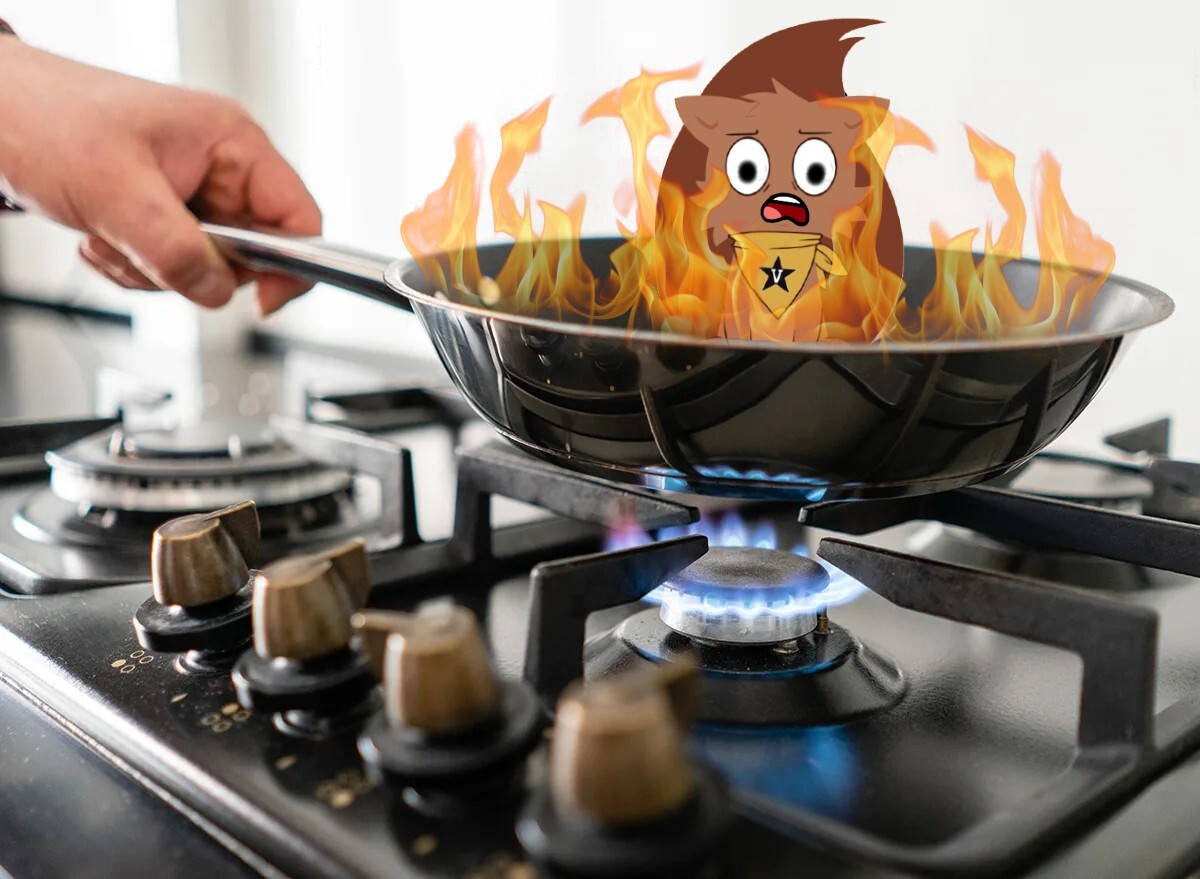
\includegraphics[scale=0.2]{FRIED_SQUIRREL.jpg}
\end{center}

\section{Introduction}
Making fried squirrel is a controversial recipe. Some people believe the squirrels deserve it. Vanderbilt University is a plentiful source of meat.

\section{Ingredients}
\begin{center}
    \begin{tabular}{|c|c|c|}
    \hline
    S.No. & Ingredient & Qty.\\
    \hline \hline
       1  &  Squirrel* & 3-5 \\
       \hline
    2 & Olive Oil & 2 tbsp. \\
    \hline
    3 & Garlic & 2-3 cloves \\
    \hline
    4 & Paprika & 2 tsp. \\
    \hline
    5 & Handkerchief (\textit{small}) & 1 \\
    \hline
    \end{tabular}
\end{center}

*deceased.

\newpage

\section{Preparation}
\begin{enumerate}
    \item Remove the fur and dice the squirrels in a bowl.
    \item Heat up the olive oil in a pan.
    \item Dry rub the squirrel with paprika and minced garlic for 30 minutes.
    \item Put the handkerchief around your wrist.
    \item Fry the rubbed squirrel in oil for 2 minutes.
    \item Serve warm with freshly squeezed lemonade.
\end{enumerate}


\end{document}
